\chapter{Timer Overview }

A hardware timer is a digital counter that:

\begin{itemize}
    \item counts regular events, normally using a fixed frequency clock source
    \item increments or decrements at a fixed frequency
    \item resets itself when reaching zero, or a predefined value
    \item generates an interrupt when reset
\end{itemize}

A software timer is a function block implemented in software:

\begin{itemize}
    \item usually based on a hardware timer, increments/decrements when interrupted
    \item provides lower time precision
    \item can have multiple instances, notably more than hardware timers
\end{itemize}


\section{Timer use-cases}

Timers can be used to:

\begin{itemize}
    \item[] generate periodic events
    \item[] measure time passed to perform some computational tasks
    \item[] generate pulse width modulation
\end{itemize}

\section{Components of a Standard Timer}

A timer is made of multiple components:

\begin{itemize}
    \item \textbf{Clock source/Oscillator}
    \item \textbf{Prescaler}
    \begin{itemize}
        \item[] Takes the clock source as input
        \item[] Divides the input frequency by a predefined value (4, 8, 16...)
        \item[] Outputs the divided frequency to other components
    \end{itemize}
    \item \textbf{Timer Register}
    \begin{itemize}
        \item[] Is incremented or decremented at a fixed frequency, taken from the prescaler
        \item[] Is driven by the output from the prescaler, often referred to as "ticks"
    \end{itemize}
\end{itemize}


\subsection{Prescalers and software performance}

Prescalers significantly improve system performance when there is a need to:

\begin{itemize}
    \item reduce power consumption
    \item count longer time intervals
    \item In real-time systems, the choice of prescalers should be carefully considered as to meet critical timing requirements
\end{itemize}


\section{Timer Operation Modes}

A standard timer typically has three operation modes.

\subsection{Compare Mode}

The compare mode has a compare register.
The compare register is loaded with a value that is periodically compared with the value in the timer
register.

Once the two values are the same an interrupt can be generated (e.g. every 15 seconds).


\begin{figure}[H]
    \centering
    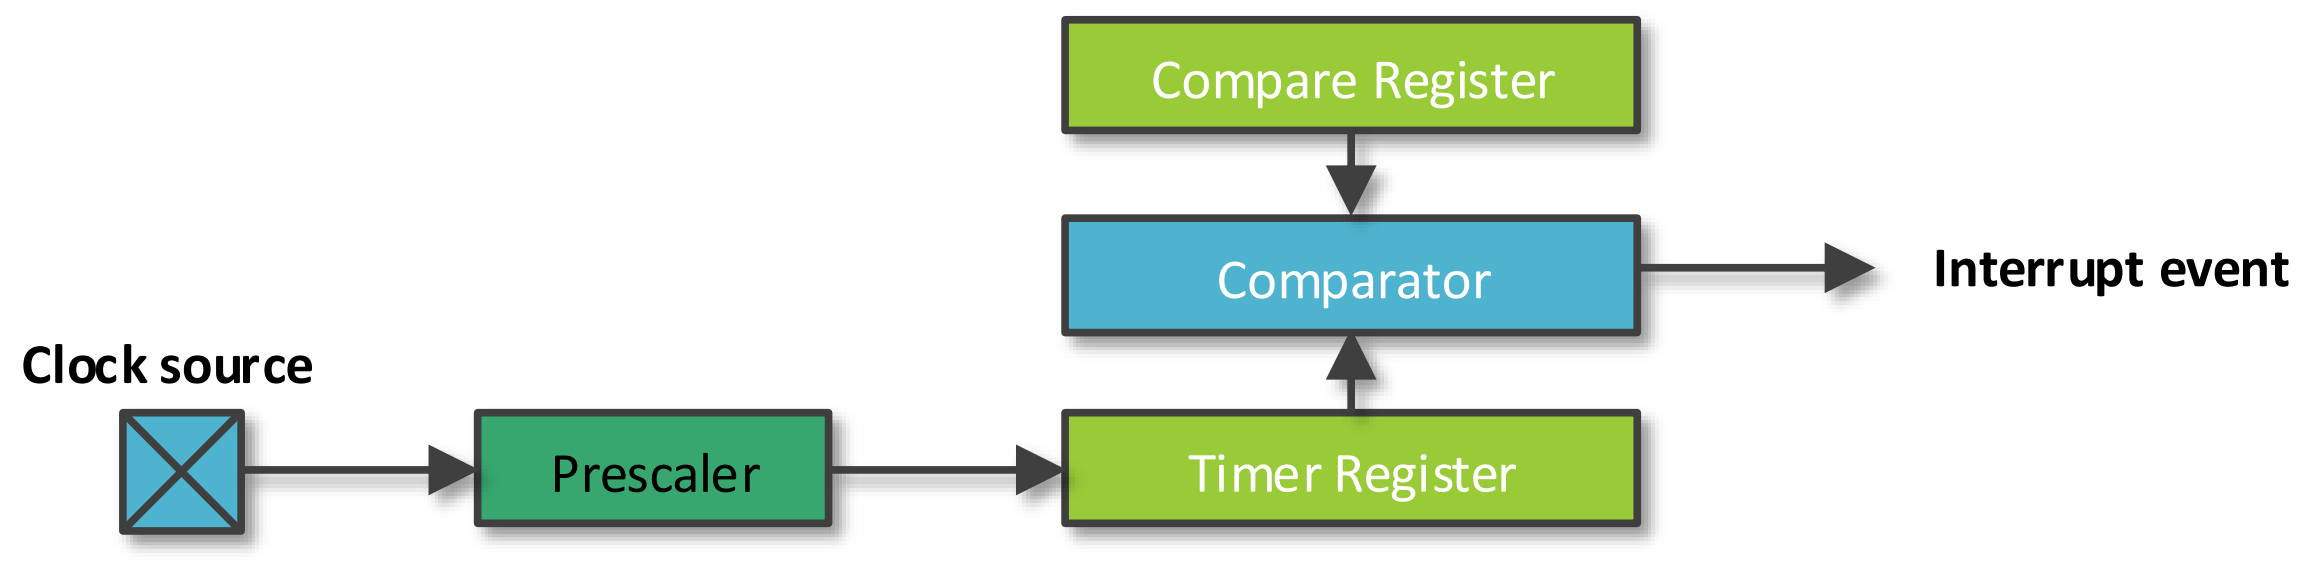
\includegraphics[width=0.75\linewidth]{img/image65.png}
\end{figure}

\subsection{Capture Mode}
The capture mode has a capture register that captures the current value of the timer register upon the
capture of external events. It can also generate an interrupt.

Optionally, the prescaler can be used to divide the frequency of the events.


\begin{figure}[H]
    \centering
    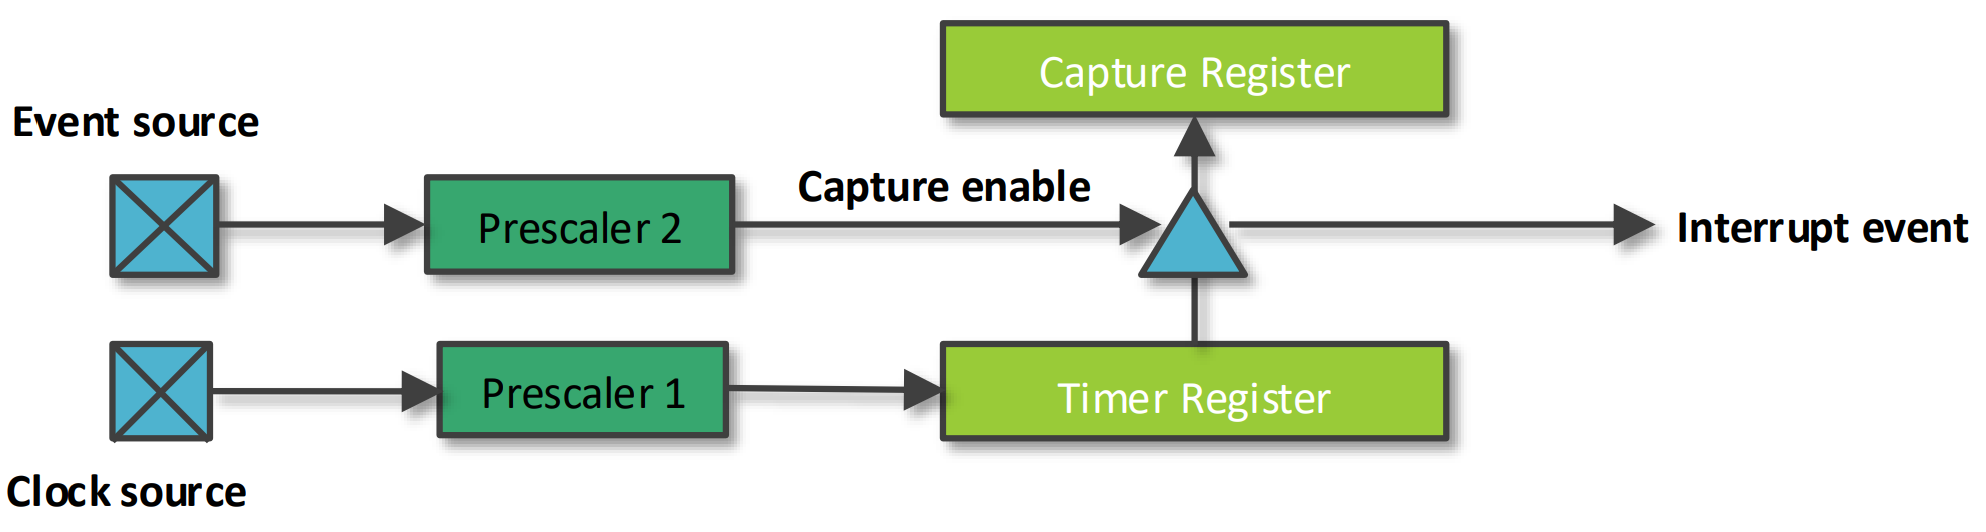
\includegraphics[width=0.75\linewidth]{img/image66.png}
\end{figure}

\subsubsection{Capture/Compare Registers}
Capture/Compare Registers, also known as CCRs, are registers used to configure and control various
timer-related functionalities. They are registers within the timer module.


\subsection{Pulse-width modulation (PWM) Mode}

This mode uses the width of a pulse to modulate an amplitude, which reflects the duty cycle, which
describes the proportion of the 1 state in one pulse period.

The PWM mode is mainly used to control the power supplied to electrical devices (via on-off intervals).

\begin{figure}[H]
    \centering
    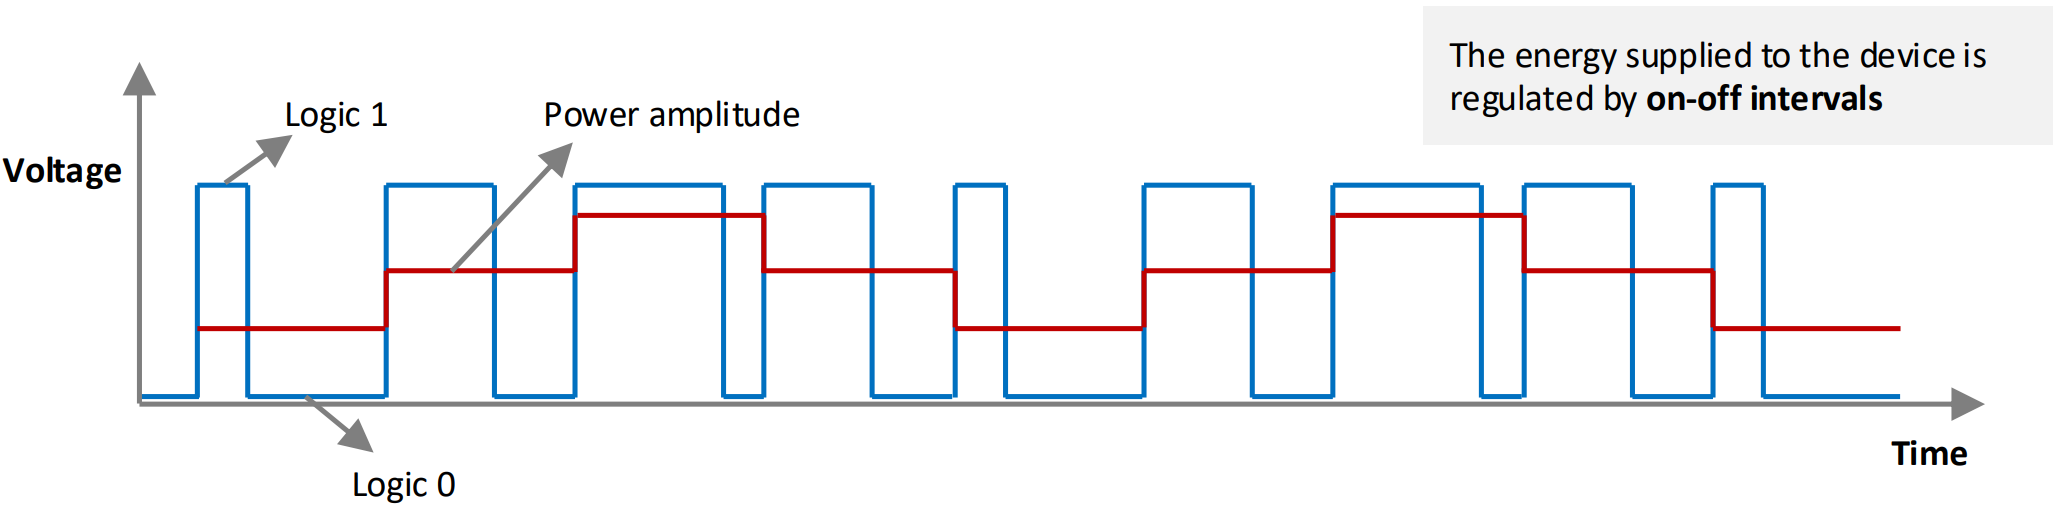
\includegraphics[width=0.75\linewidth]{img/image67.png}
\end{figure}

\section{MSP432 Timer A}
In our launchpad are 4 16-bit timers: TA0, TA1, TA2, TA3. Each one has 7 capture/compare registers,
allowing software timers.

There are TAxR registers that can be manipulated. They can be cleared by setting the TACLR bit.

The timer clock can be sourced from: ACLK, SMCLK, or externally from TAxCLK or INCLK. The clocks
are connected to crystal oscillators. The clock source is selected with the TASSEL bits.
\paragraph{}
The selected clock source may be passed directly to the timer, or it can be slowed down by 2, 4, 8 using
ID bits. Or 2, 3, 4, 5, 6, 7, 8 using TAIDEX bits.

\begin{figure}[H]
    \centering
    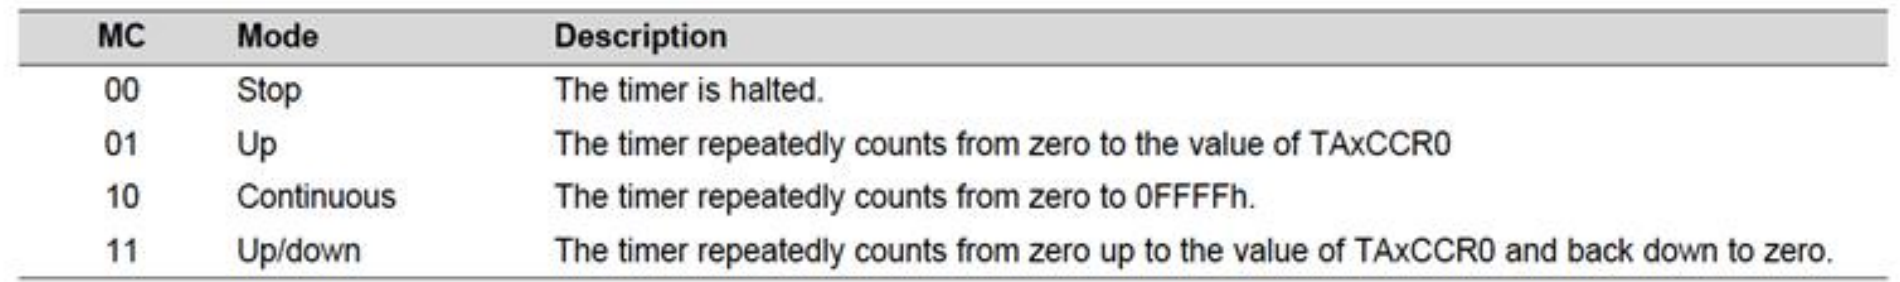
\includegraphics[width=0.75\linewidth]{img/image68.png}
\end{figure}

\subsection{Up Mode}
In Up Mode the timer repeatedly counts up to the value of the compare register, TAxCCR0.
Once the two values match the TAxCCR0 CCIFG (capture compare register interrupt flag) is set.
We need to enable the interrupt first. We do this via the CCIE bit in the TAxCCTL0 (Capture/Compare
Control Register) register.

\begin{figure}[H]
    \centering
    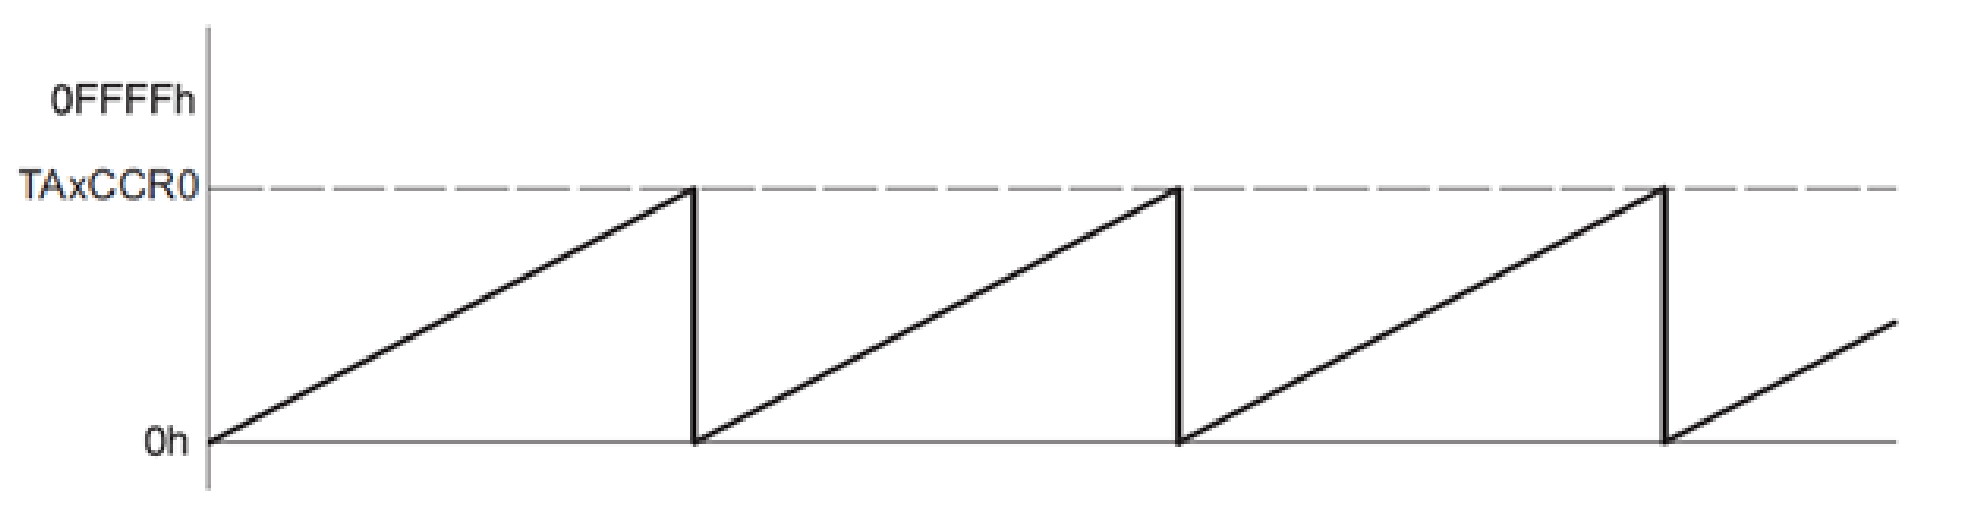
\includegraphics[width=0.75\linewidth]{img/image69.png}
\end{figure}

\section{Periodic timer interrupt setup}

We first set the CCIE (Capture Compare Interrupt Enable) bit in TA0 CCTL0 register to enable interrupt.
\begin{lstlisting}[language=c++]

    TIMER_A0->CCTL[0] = TIMER_A_CCTLN_CCIE;

\end{lstlisting}

\paragraph{We are using the first capture/compare register of the first timer A.}

Then we set the value for the comparison.

\begin{lstlisting}[language=c++]

    TIMER_A0->CCTL[0] = TIMER_A_CCTLN_CCIE;
    TIMER_A0->CCR[0] = 50000;
    TIMER_A0->CTL = TIMER_A_CTL_SSEL__SMCLK | TIMER_A_CTL_MC__CONTINUOUS;
\end{lstlisting}


In this case the timer will count up to 50000.
We then set the clock source as SMCLK (3 MHz) in continuous mode.
We use the TA0CTL Control Register for this register.

\paragraph{}

We can also use an input divider (Prescaler) for SMCLK to slow down the input clock signal.
By default the SMCLK is 3 MHz, which means 3,000,000 ticks per second.
By dividing by 8, we get 375,000 ticks per second, the equivalent of 7 interrupts per second.

\begin{lstlisting}[language=c++]

    TIMER_A0->CCTL[0] = TIMER_A_CCTLN_CCIE;
    TIMER_A0->CCR[0] = 50000;
    TIMER_A0->CTL = TIMER_A_CTL_SSEL__SMCLK | TIMER_A_CTL_MC__CONTINUOUS | TIMER_A_CTL_ID_3;
    NVIC->ISER[0] = 1 << ((TA0_0_IRQn) & 31);
\end{lstlisting}

We then have to enable the timer IRQ.
There is a specific IRQ line for CCR0 (the first compare register), while all others (TA0CCR1) share the
same IRQ. Weird design choice.
To counter this (pun intended), we just need to check which CCR triggered the interrupt within the ISR to
distinguish between them.


\begin{figure}[H]
    \centering
    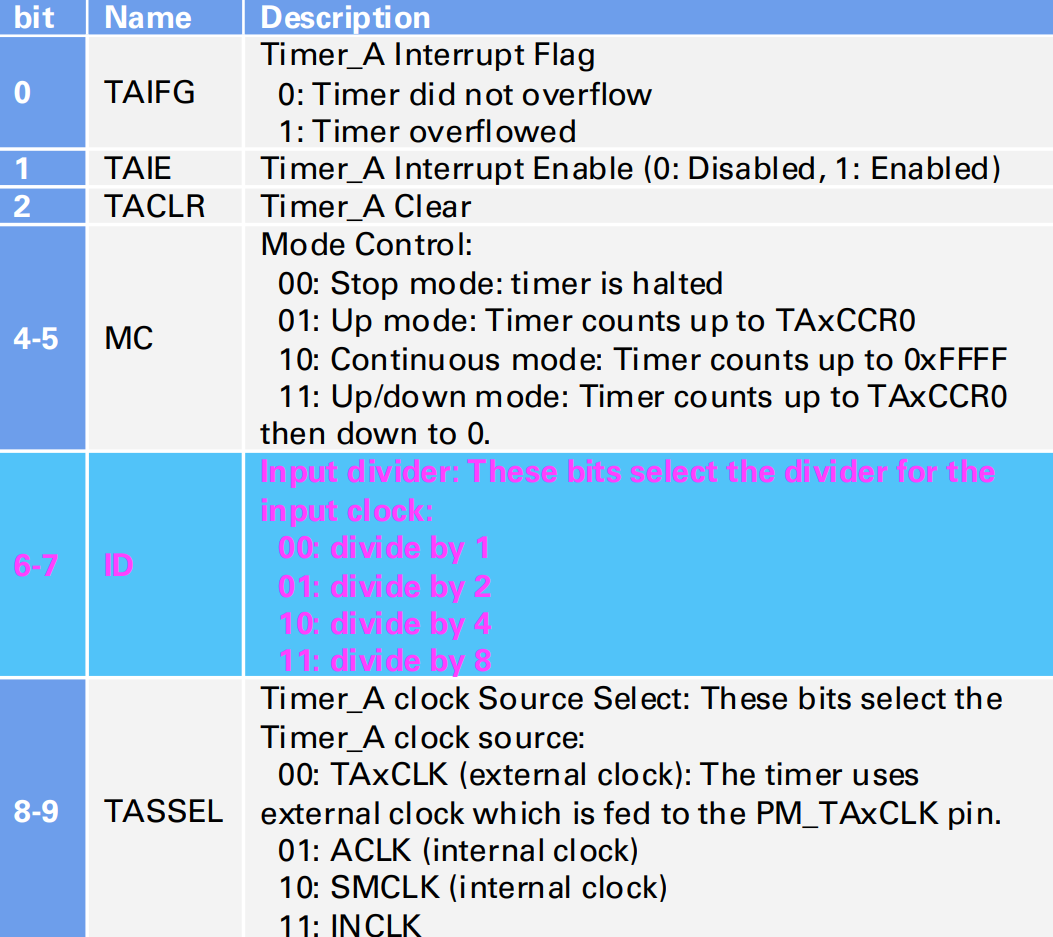
\includegraphics[width=0.6\linewidth]{img/image70.png}
\end{figure}


We then override the Timer Interrupt Handler:
\begin{lstlisting}[language=c++]

    // will be called when TA0CCR0 CCIFG is set
        void TA0_0_IRQHandler(){
        // clear the interrupt flag
        TIMER_A0->CCTL[0] &= ~TIMER_A_CCTLN_CCIFG;
        // toggle LED
        P1->OUT ^= BIT0;
    }
\end{lstlisting}

Just like the other interrupts, we clear the interrupt flag and then do our thing.

\section{Timer Overflow and Counters}
We have to keep in mind timer overflow and counters.

Timer overflows can be used with counters to measure time (e.g. count 1 second if the timer overflows 6
times).

Timer overflows happen because Time Registers have a finite count range (in MSP432 they are 32-bit).
Counters can also be used to measure performance, frequencies, duty cycles and other performance-related metrics.


\section{Watchdog Timer}

Apart from timers we have watchdog timers. Watchdog module performs a controlled system restart after
a software problem occurs/the system gets stuck.
Watchdog timer counts down from a selected interval.
If the selected time interval expires, a system reset is generated.

To edit the control register, the WDTCTL register, we have to insert the password first:


\begin{lstlisting}[language=c++]

    WDT_A->CTL = WDT_A_CTL_PW | WDT_A_CTL_HOLD
\end{lstlisting}

\section{Clocks in MSP432}

Microcontrollers usually have two types of clock resources:

\begin{itemize}
    \item \textbf{on-chip} oscillator (internal oscillator). \textbf{Advantage}: always present
    \item oscillator \textbf{connected} to external crystal (external oscillator). \textbf{Advantage}: higher precision
\end{itemize}

The clock system contains the sources of the various clocks in the device. It also controls the mapping
between the sources and the different clocks in the device.


\subsection{External clock resources:}

\begin{itemize}
    \item LFXTCLK: Low-Frequency Oscillator (LFXT) 32-kHz or below
    \item HFXTCLK: High-Frequency Oscillator (HFXT) 1-MHz to 48-MHz range
\end{itemize}

\subsection{Internal clock resources:}

\begin{itemize}
    \item DCOCLK: Internal Digitally Controlled Oscillator (DCO) Programmable frequencies (3-MHz frequency by default)
    \item VLOCLK: Internal Very-Low-Power Low-Frequency Oscillator (VLO) 9.4-kHz typical frequency
    \item REFOCLK: Internal Low-Power Low-Frequency Oscillator (REFO) Selectable 32.768-kHz or 128-kHz frequencies
    \item MODCLK: Internal Low-Power Oscillator 25-MHz typical frequency
    \item SYSOSC: Internal Oscillator 5-MHz typical frequency
\end{itemize}


\paragraph{Five primary system clock signals are available from the clock module:}

\begin{itemize}
    \item[] ACLK (Auxiliary Clock)
    \item[] MCLK (Master Clock) -> To CPU
    \item[] HSMCLK (Subsystem Master Clock)
    \item[] SMCLK (Low-Speed Subsystem Master Clock)
    \item[] BCLK (Low-Speed Backup Domain Clock)
\end{itemize}

The clock system can be configured or reconfigured by software at any time during program execution.
We have selection and divider signals.


\begin{figure}[H]
    \centering
    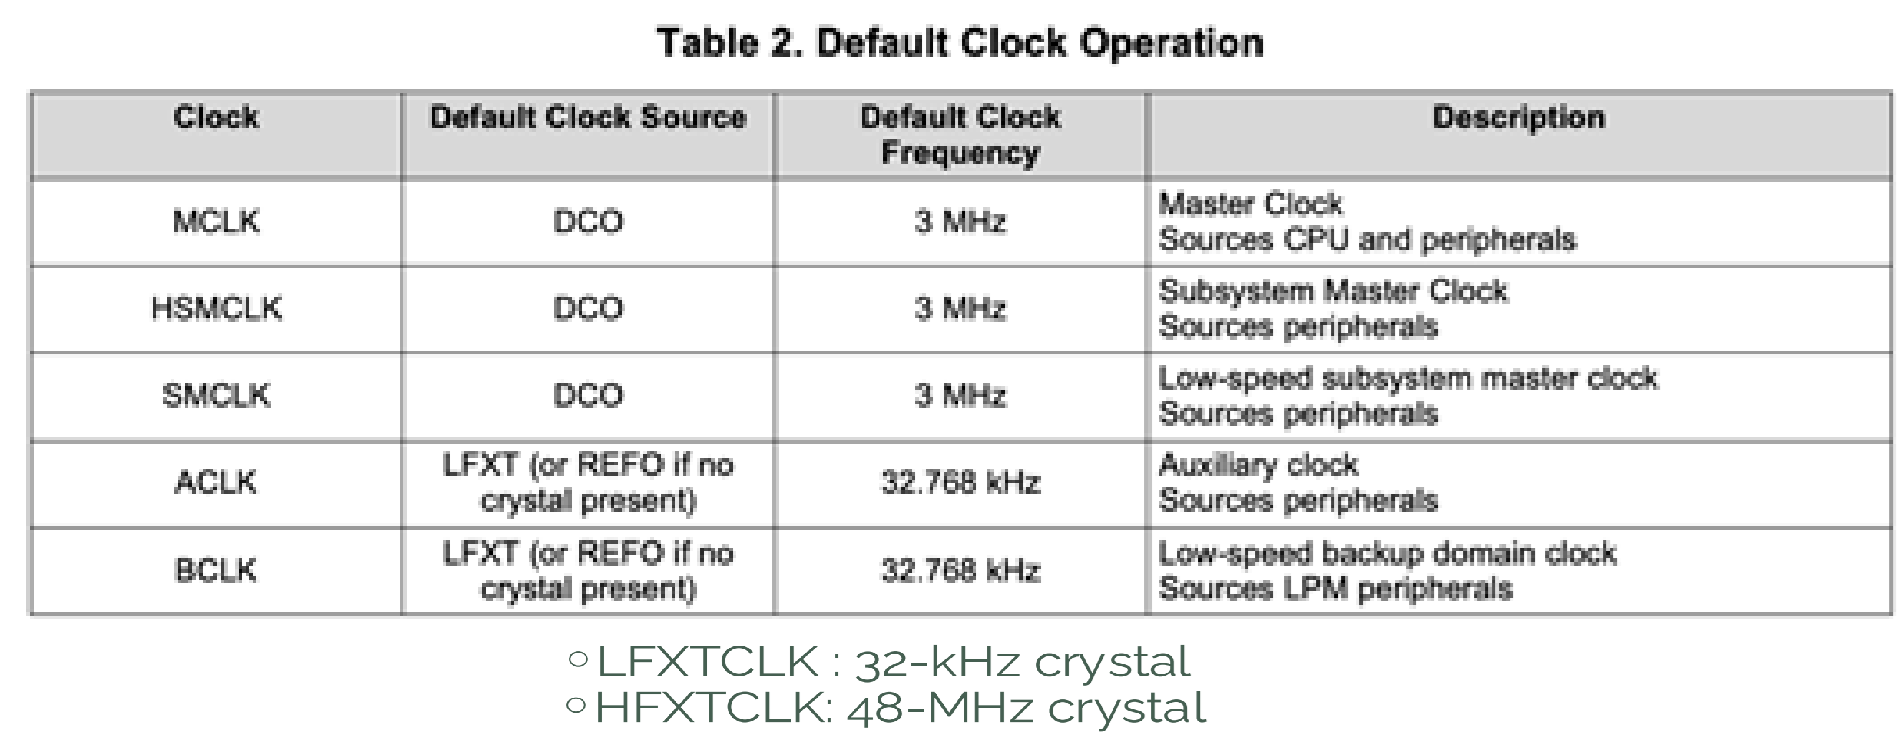
\includegraphics[width=0.75\linewidth]{img/image80.png}
\end{figure}

\subsubsection{Example Configuration}

We first need to unlock the CS module for register access, which is protected by password to prevent
inadvertent access.

\begin{lstlisting}[language=c++]

   CS->KEY = CS_KEY_VAL;
    CS->CTL1 |= CS_CTL1_SELA_2 | CS_CTL1_SELS_3 | CS_CTL1_SELM_3
    CS->KEY = 0;
\end{lstlisting}


We could also use a divider to slow down the CPU frequency, by doing this:

\begin{lstlisting}[language=c++]

   CS->KEY = CS_KEY_VAL;
    CS->CTL1 |= CS_CTL1_SELA_2 | CS_CTL1_SELS_3 | CS_CTL1_SELM_3 | CS_CTL1_DIVM_7
    CS->KEY = 0;
\end{lstlisting}


This way we divide the Master Clock signal by $128$.
The DCO by default is $3 MHz$, so it's reduced to $23,437.5 Hz$


\subsection{Slowing CPU to the smallest frequency possible}

We can do this by setting the Master Clock to use the DCO then set the DCO's frequency to 1.5 MHz then
divide it by 128. We achieve $\sim24 kHz$ by doing so.
Or we can set the Master Clock to use VLOCK, which is 9.5 kHz.